\documentclass[a4paper,12pt]{report}
\usepackage[a4paper,inner = 1.7cm, outer = 2.7cm, top = 2cm, bottom = 2cm, bindingoffset = 1.2cm]{geometry}

\usepackage[english]{babel}
\usepackage{blindtext}
\usepackage{fancyhdr}
\usepackage{wrapfig}
\usepackage{graphicx}

\fancyhf{}
\renewcommand{\headrulewidth}{2pt}
\renewcommand{\footrulewidth}{1pt}
\fancyhead[LE]{\leftmark}
\fancyhead[RO]{\rightmark}
\linespread{1.25}
\hyphenpenalty=5000
\begin{document}
\begin{center}
\pagestyle{empty}
       \vspace*{1cm}

       \textbf{UNIVERSITATEA DIN BUCUREȘTI
FACULTATEA DE MATEMATICĂ ȘI INFORMATICĂ}

       \vspace{0.5cm}
        LUCRARE DE LICENȚĂ
            
       \vfill
           
       \vspace{0.8cm}
\textbf{Coordonator:}
\hfill
\textbf{Absolvent:} \\
\textbf{Prof. Dr. Radu Ionescu}
\hfill
\textbf{Moldovan George-Alexandru} \\

\vspace{0.8cm}
      București \\
Iunie (fingers crossed), 2020
\clearpage         
\end{center}
\newpage

\begin{center}
\pagestyle{empty}
       \vspace*{1cm}

       \textbf{UNIVERSITATEA DIN BUCUREȘTI
FACULTATEA DE MATEMATICĂ ȘI INFORMATICĂ}

       \vspace{0.5cm}
        Sistem pentru detectarea anomaliilor in video
            
       \vfill
           
       \vspace{0.8cm}
\textbf{Coordonator:}
\hfill
\textbf{Absolvent:} \\
\textbf{Prof. Dr. Radu Ionescu}
\hfill
\textbf{Moldovan George-Alexandru} \\
    
\vspace{0.8cm}  
	București \\
Iunie (fingers crossed), 2020
\clearpage
\end{center}
\newpage

\tableofcontents
\pagenumbering{arabic}
\setcounter{page}{2}
\begin{abstract}
\par Având în vedere contextul actual, detectarea anomaliilor în video este un subiect de interes în mai multe arii, în mod special in securitatea publică. Putem spune ca această problemă este încă nerezolvată, deoarece sistemele actuale, deocamdată, nu depăşesc  omul cand vine vorba de detectarea anomaliilor. De asemenea, o altă problemă a sistemelor de detectare a anomaliilor în video este nevoia acestora de resurse computaţionale mari in partea de inferența, facând aproape imposibilă rularea acestora direct pe hardware-ul existent al sistemelor de supraveghere video actuale, acolo unde acestea prezinta un maxim interes. Astfel, putem spune că dezvoltarea unui sistem capabil să transforme sistemele de supraveghere actuale în sisteme ce pot recunoaşte evenimente anormale  este un subiect ce poate revoluţiona domeniului supravegherii video. Această lucrare îşi propune o implementare al sistemului state-of-the-art la momentul redactării, aşa cum este prezentat de \emph{Ionescu et al.} \cite{ionescu2019object}. Obiectivul este obţinerea unei arhitecturi ce foloseşte o soluţie PaaS si expunerea etapei de inferenţă printr-un API astfel încât convertirea unui sistem de supraveghere clasic într-unul inteligent să devină doar o problemă de implementare, fara a fi nevoie de schimbarea hardware-ului. Utilizarea unei soluţii PaaS pentru etapa de inferenţă rezolvă problema executării cererilor fară complexitatea creeri si intreţinerii unei infrastructuri de maşini virtuale sau fizice. 
\end{abstract}

\chapter{Introducere}
\section{Motivatie}
\quad Detectarea anomaliilor in video este in strânsă legatură cu sistemele de supraveghere inteligente,un domeniu care a fost si este de interes pentru mine. La rândul lor, sistemele de supraveghere inteligente, au o mare importanţă in securitatea publică. Cu toţii ne dorim o lume in care apelurile de urgenţă in caz de incendiu se fac automat, alunecările de teren sunt descoperite înainte să fie prea târziu, iar oamenii rău intenţionaţi sunt opriţi inainte să se întâmple tragedii. 
\par
Astfel, arhitectura folosită se bazează pe detecţia caracteristicilor spaţio-temporale ale evenimentelor prezente în video, care mai apoi sunt împărţite in clase de normalitate. Aceste caracteristici sunt extrase trecând evenimentul printr-o serie de autoencodere pentru a folosi mai apoi reprezentarea latentă in cadrul clasificării finale. In etapa de antrenare, se folosesc filmări ce prezintă comportamentul normal in scenariul analizat. Analizând aceste video-uri putem creea un model capabil să recunoască dacă un eveniment aparţine unei clase de normalitate analizate pana acum, sau dacă este un caz anormal. Deoarece un eveniment poate fii ales in multe moduri, în cadrul acestui sistem un eveniment reprezintă orice obiect aflat în cadru. Analiza asupra fiecarui obiect conţine şi un cadru precedente dar si unul viitor, asemănator cu modalitatea folosită de \emph{Ionescu et al.}  \cite{ionescu2019object}. O menţiune in acest sens ar fi că deoarece pentru fiecare obiect sunt analizate si cadrele de la pozitie t-3 si t+3  respectiv la poziţia t a cadrului analizat, atunci cand sistemul va analiza un video in sistem live-feed, analiza se va face cu un decalaj de 3 cadre. Având în vedere ca pentru un video actual viteza de redare este de minim 15 cadre pe secundă, acest decalaj este neglijabil.
\par
Pe lângă partea algoritmica a detectării anomaliilor, o alta arie de interes a acestei lucrări este cloud computing. Această parte analizează un nou mod de rulare, ce facilitează atât dezvoltarea cât si execuţia ulterioară a unor sisteme complexe. Acest nou mod constă in folosirea unei arhitecturi plasată în cloud, ce oferă dezvoltatorului posibilitatea să creeze sisteme ce necesită multe resurse in timpul rulării, fara costurile asociate creeri si menţinerii unei infrastructuri proprii. Pe de altă parte, având in vedere că toate operaţiunile sunt executate in cloud, utilizatorii serviciului au nevoie doar de conexiune la internet şi cerinţe minime pentru sistemele proprii, fara a fi nevoiţi să achiziţioneze echipamente noi pentru a folosi sisteme de detecţie a anomaliilor.
\section{Context}
\quad Detectarea anomaliilor in video poate fi văzută ca o problemă subiectivă, deoarece un eveniment este normal sau anormal doar dacă este luat în considerare şi contextul în care acesta apare. Un exemplu foarte bun este lupta între două persoane si o persoană care se plimbă. Care dintre aceste evenimente este anormal ? Desigur, depinde de context. Dacă sistemul supraveghează o arena de lupte, atunci persoana care se plimbă in ring prezintă un comportament anormal, in timp ce luptătorii prezintă comportamentul aşteptat. Din acest motiv majoritatea lucrărilor din domeniu \cite{cheng2015,ionescu2019object,sultani2018}...  abordează un mod de lucru bazat pe antrenarea folosind video-uri ce provin din aceeasi locaţie cu cele de test. Tocmai din cauza dependenţei de context, detectarea anomaliilor nu este o problemă ce poate fi generalizată, astfel fiecare scenariu necesită o antrenare si un model propriu. \par

Ca şi moduri de expunere a soluţiei software catre utilizatori, aceasta se poate face in 2 moduri :
\begin{itemize}
\item Folosind servere proprii
\item Folosind servicii cloud
\end{itemize}
\par
Folosirea serverelor proprii presupune, pe lângă prezenţa fizică a serverelor şi cumpărarea tuturor serviciilor conexe, cum ar fi servere de baze de date, sisteme de distribuire a fişierelor, infrastructură de reţea, ş.a.m.d., este nevoie si de o echipă dedicată pentru intreţinerea infrastructurii si repararea eventualelor probleme ce pot apărea. Aceste considerente, împreuna cu faptul că scalarea soluţiilor software este foarte anevoioasă atunci când este folosită infrastructura proprie, fac această soluţie să nu mai fie folosită în mod curent deoarece incetineşte modul de dezvoltare a aplicaţiei, iar rezultatul final este si el unul mai puţin calitativ decât ce se poate obţine folosind soluţii în cloud. 
\par
\begin{wrapfigure}{r}{0.45\textwidth}
    \begin{center}
        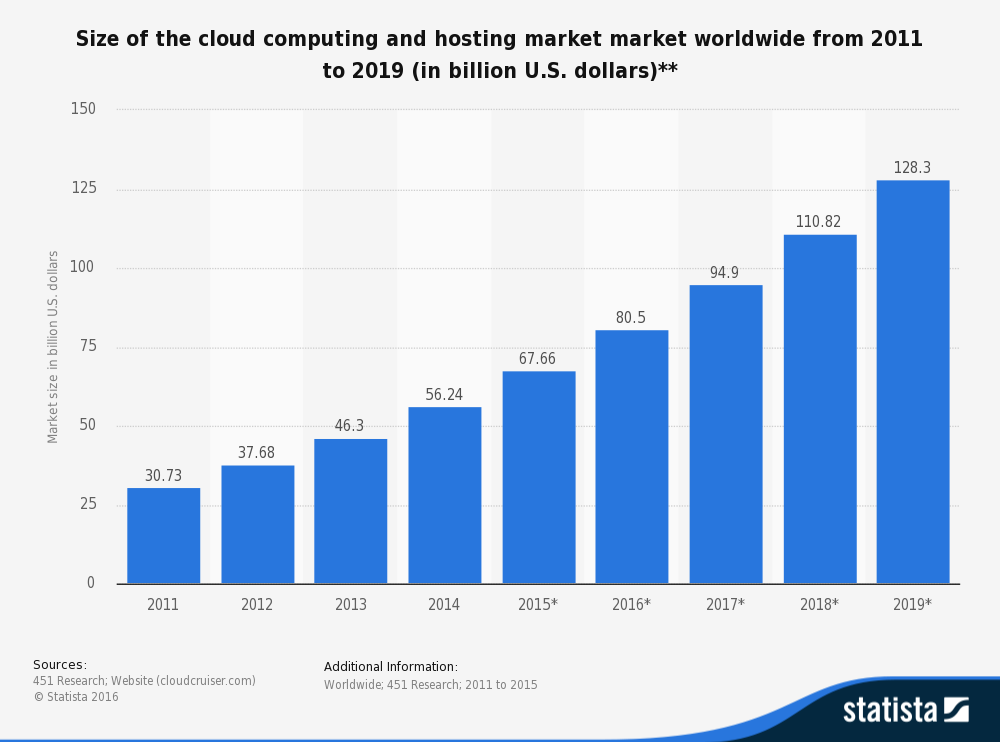
\includegraphics[width=0.4\textwidth]{images/grafic_cloud_computing}
			\label{fig:cloud_computing_graph}
    \end{center}
\end{wrapfigure}
Folosirea serviciilor cloud oferă multiple posibilităţi de dezvoltare a aplicaţiilor, de la creeare unei infrastructuri complete care este administrată în totalitate de către dezvoltator, la medii de execuţie serverless care sunt complet administrate de către provider-ul de servicii cloud. 
Deşi creearea unei infrastructuri proprii înca este necesară acolo unde legislaţia nu permite ca datele sa fie stocate in cloud, în toate celelalte cazuri se face migrarea spre soluţii cloud, lucru vizibil si in evoluţia cotei de piata a domeniului cloud-computing la nivel global, aşa cum se poate observa si in ~\ref{fig:cloud_computing_graph}. 


\section{Conţinutul lucrării}
 Ca şi structură, lucrarea este impărţita in 2 parţi:
\begin{itemize}
\item Partea algoritmica a sistemului de detectare a anomaliilor in video
\item Partea de deployment a sistemului
\end{itemize}
\par În prima parte sistemul va fi analizat si detaliat din punct de vedere algoritmic si teoretic studiind problema detectiei propriu zisă. Ca şi tehnologii, in această parte am ales sa folosesc Python3 ca şi limbaj de programare pentru anvantajele pe care le are. Printre acestea se numără faptul ca este un limbaj orientat pe obiecte care pune la dispozitia dezvoltatorului numeroase librării specifice pentru AI/ML mutând astfel atenţia dinspre detalii de implementare spre detalii de arhitectura şi probleme mai abstracte ale programului care sunt cu adevărat importante pentru rezultatul final. Una dintre librăriile care s-a dovedit esenţială dezvoltarii este \emph{Keras} \cite{2020keras}, care oferă un API ce uşurează dezvoltarea unei reţele neuronale adânci/convoluţionale dar şi optimizează timpul de antrenare pentru modelele create.  \par
În cea de a doua parte este analizat tipul de deployment al aplicaţiei. Aici vor fi prezentate analize detaliate ale avantajelor si dezavantajelor soluţiilor cloud, dar si motivele pentru care modul final de deployment a fost ales. \\
Soluţiile de cloud-computing analizate vor fi:
\begin{itemize}
\item Infrastructure as a Service (IaaS) - analiză pe Amazon EC2
\item Platform as a Service (PaaS) - analiză pe Amazon Elastic Beanstalk
\item Function as a Service (FaaS) - analiză pe Amazon Lambda
\end{itemize}
\chapter{Plictiseala}
In ceea ce priveşte FaaS, acesta este un domeniu nou, deoarece a apărut pentru prima data in 2010 fiind oferit de câteva start-upuri la acea vreme. Acest mod de dezvoltare orientat spre microservicii a devenit trendul in industrie în ultimii ani pentru sisteme cu potenţial de scalare mare, deoarece prezintă numeroase avantaje din punct de vedere al modului de dezvoltare si de executie in industrie. In momentul de faţă, pentru servicii de tip FaaS sunt 3 mari jucători: Amazon cu AWS Lambda, Google cu Google Cloud Functions si Microsoft cu Azure Functions.\cite{jonas2019cloud}. Numeroase lucrări din domeniu \cite{christidis2019, wang2019} arată ca rularea algoritmilor de machine learning folosind soluţii FaaS (Function as a service) precum AWS Lambda sau Google cloud functions, este în sine o problemă ce necesită soluţii de optimizare a codului pentru a indeplini restricţiile soluţiilor de rulare serverless, cum ar fi memoria limitată a mediului de execuţie. 
\blindtext[3]

\bibliographystyle{abbrv}
\bibliography{References}
\end{document}